\chapter{Медленные системы}

\

Возьмём известную нам "быструю систему", и добавим ограничение на скорость конвейера: введём множество $\mathbb{V}$  допустимых скоростей $v_i$, каждая из которых является вполне конечной. Например, в Satisfactory: 

\noindent $\mathbb{V} = \{60, 120, 270, 480, 720, 1200\}$. Тогда необходимо помимо абстрактной площади начать учитывать и длину конвейеров. А так же необходимо начать учитывать взаимодействие ресурсов и время этого взаимодействия.

\

Обычно, в играх по типу Satisfactory и Factorio "скорость" конвейера измеряется не в метрических единицах $[v_i]$ = м/с, а как пропускная способность $[q_i]$ = шт/с. Но одно можно перевести в другое, если добавить плотность ёмкости конвейера $[\rho_i]$ = шт/м. $v_i \cdot \rho_i = q_i$

\

Однако это всё не меняет допустимый набор действий, а просто накладывает на него некоторые ограничения, и меняет суть задачи: мы перераспределяем не просто ресурсы, а пропускные способности.

$$
\left[
\begin{matrix}
	m_{11} & \ldots & m_{1n} \\
	\vdots & \ddots & \vdots \\
	m_{k1} & \ldots & m_{kn}
\end{matrix}
\right]
\times
\left[
\begin{matrix}
	q^{\text{in}}_1 \\
	\vdots \\
	q^{\text{in}}_n
\end{matrix}
\right]
=
\left[
\begin{matrix}
	q^{\text{out}}_1 \\
	\vdots \\
	q^{\text{out}}_n
\end{matrix}
\right]
$$

\

В матричной форме преобразования, элементы самой матрицы -- скаляры, а элементы векторов -- пропускные способности $[q_i]$ = шт/с

\

Важно отметить, что пропускная способность \underline{конвейера} $q_i$ и пропускная способность \underline{русурсов} $q^{\text{res}}$ -- это две разные, но взаимосвязные вещи: $q^{\text{res}}$ -- это то, что производят заводы, и что "выливается" на конвейеры, которые двигаются с $v_i$, и имеют $\rho_i$. Для адекватной работы такой системы необходимо, чтобы $q^{\text{res}} \le q_i$. В противном случае завод не сможет выкладывать ресурсы на конвейер -- то есть будет простаивать. Таким образом, схемы необходимо проектироавть с учётом этих двух величин.

\

Если же $q^{\text{res}} > q_i$ -- то возможны 2 принципиальные ситуации: $q_i = 0$ и $q_i \ne 0$. Рассмотрим первую на двух примерах:






\vspace{0.25in}
\section{Тупики}







\

\begin{minipage}{0.5\textwidth}
	\begin{tikzpicture}[
		s/.style = {rectangle, draw=blue!60,	fill=blue!5,	very thick, minimum size=20},
		a/.style = {rectangle, draw=red!60,		fill=red!5,		very thick, minimum size=20},
		o/.style = {rectangle, draw=green!60,	fill=green!5,	very thick, minimum size=20},
		r/.style = {->, thick, rounded corners=10pt},
		]
		
		% === === Nodes === ===
		\node[o]	(in)	at	(0, 2)	{in};
		\node[s]	(s)		at	(0, 0)	{s};
		\node[o]	(out2)	at	(0, -2)	{out};
		\node[o]	(out3)	at	(2, -2)	{out};
		\node[
			regular polygon, regular polygon sides=6, 
			draw, draw=red!60, fill=red!40, 
			very thick, minimum size=1cm
			] (out1) at (-2, -2) {};
		\draw[
			rounded corners=1.25pt,
			draw, draw=white!100, fill=white!100
			] (-2.25, -2.1) rectangle (-1.75, -1.9);
		
		
		
		% === === Lines === ===
		\draw[r]	(in.south)	to	node[right]	{$q$}	(s.north);
		\draw[r]	(s.west)	-|	node[above]	{$0$}	(out1.north);
		\draw[r]	(s.south)	to	node[right]	{$q/2$}	(out2.north);
		\draw[r]	(s.east)	-|	node[above]	{$q/2$}	(out3.north);
		
	\end{tikzpicture}
\end{minipage}
\begin{minipage}{0.5\textwidth}
	\begin{tikzpicture}[
			s/.style = {rectangle, draw=blue!60,	fill=blue!5,	very thick, minimum size=20},
			a/.style = {rectangle, draw=red!60,		fill=red!5,		very thick, minimum size=20},
			o/.style = {rectangle, draw=green!60,	fill=green!5,	very thick, minimum size=20},
			r/.style = {->, thick, rounded corners=10pt},
			]
			
			% === === Nodes === ===
			\node[o]	(in)	at	(0, 4)		{in};
			\node[s]	(s1)	at	(0, 2)		{s};
			\node[s]	(s2)	at	(-2, 0)		{s};
			\node[s]	(s3)	at	(2, 0)		{s};
			\node[o]	(out2)	at	(-1, -2)	{out};
			
			\node[
				regular polygon, regular polygon sides=6, 
				draw, draw=red!60, fill=red!40, 
				very thick, minimum size=1cm
				] (out1) at (-3, -2) {};
			\draw[
				rounded corners=1.25pt,
				draw, draw=white!100, fill=white!100
				] (-3.25, -2.1) rectangle (-2.75, -1.9);
			
			\node[o]	(out3)	at	(1, -2)	{out};
			\node[o]	(out4)	at	(3, -2)	{out};
			
			
			
			
			% === === Lines === ===
			\draw[r]	(in.south)	to	node[right]	{$q$}	(s1.north);
			\draw[r]	(s1.west)	-|	node[above]	{$q/2$}	(s2.north);
			\draw[r]	(s1.east)	-|	node[above]	{$q/2$}	(s3.north);
			\draw[r]	(s2.west)	-|	node[above]	{$0$}	(out1.north);
			\draw[r]	(s2.east)	-|	node[above]	{$q/2$}	(out2.north);
			\draw[r]	(s3.west)	-|	node[above]	{$q/4$}	(out3.north);
			\draw[r]	(s3.east)	-|	node[above]	{$q/4$}	(out4.north);
		
	\end{tikzpicture}
\end{minipage}






\vspace{0.5in}

Если все конвейеры (кроме тупикового) способны полностью перевозить поданные ресурсы, а спиттеры работают мгновенно -- то сплиттер, подключённый к тупиковой ветке просто уменьшает период своей циклической группы на 1: 

$$C[t_i] \xrightarrow{\text{deadend}} C[t_i-1]$$

\

Таким образом тупик можно интерпретировать, как конвейерный разделитель с нулевым количеством выходов, а следовательно, он -- пустая циклическая группа $C[0]$.

\

Однако важно понимать, что уменьшается период лишь одного сплиттера, а не всей системы целиком, что отлично видно на второй схеме.

\

Благодоря тупиковым ветвям, можно получить преобразование: $\mathbb{T} \to \{ 2, 3 \ldots, \text{max}(\mathbb{T}) \}$, что упрощает построение многих схем.









\vspace{0.25in}
\section{Избыток на выход}

\







\noindent Рассмотрим теперь вторую ситуацию: $q^{\text{res}} > q_i$:

\vspace{0.5in}

\begin{tikzpicture}[
	s/.style = {rectangle, draw=blue!60,	fill=blue!5,	very thick, minimum size=20},
	a/.style = {rectangle, draw=red!60,		fill=red!5,		very thick, minimum size=20},
	o/.style = {rectangle, draw=green!60,	fill=green!5,	very thick, minimum size=20},
	r/.style = {->, thick, rounded corners=10pt},
	r2/.style = {line width=1pt, 
		double distance=1pt, 
		arrows = {-Stealth[inset=0pt, angle=45:10pt]},
		rounded corners=10pt,
		red
	},
	]
	
	% === === Nodes === ===
	\node[o]	(in)	at	(0, 2)		{in};
	\node[s]	(s)		at	(0, 0)		{s};
	\node[o]	(out1)	at	(-1, -2)	{out};
	\node[o]	(out2)	at	(1, -2)		{out};
	
	\draw[fill=black, thick] (-2,4) circle (3pt) node[right] {$\ q_0>>q$};
	\draw[fill=white, draw=red, thick] (-2,3) circle (3pt) node[right] {$\ q_1 < q/2$};
	
	
	
	% === === Lines === ===
	\draw[r]	(in.south)	to	node[right]	{$q$}	(s.north);
	\draw[r2]	(s.west)	-|	node[above]	{$q_1$}	(out1.north);
	\draw[r]	(s.east)	-|	node[above]	{$q-q_1$}	(out2.north);
	
\end{tikzpicture}



\vspace{0.5in}

Работает данная схема так: если $q_1 \ge q/2$ -- то разделитель работает по обычным правилам. В противном же случае появляется новое правило: разделитель первый цикл работает как $C[t_i]$ вплоть до посещения "критического" выхода. Как только до него доходят -- запускается таймер на $1/q_1$, и пока он не истечёт -- считается, что на этом выходе -- тупик - то есть $C[t_i] \to C[t_i-1]$

\

\noindent Иллюстрация того, \textbf{насколько} сильно может измениться суть схемы, если поставить другой конвейер:




\vspace{0.5in}

\begin{minipage}{0.5\textwidth}
	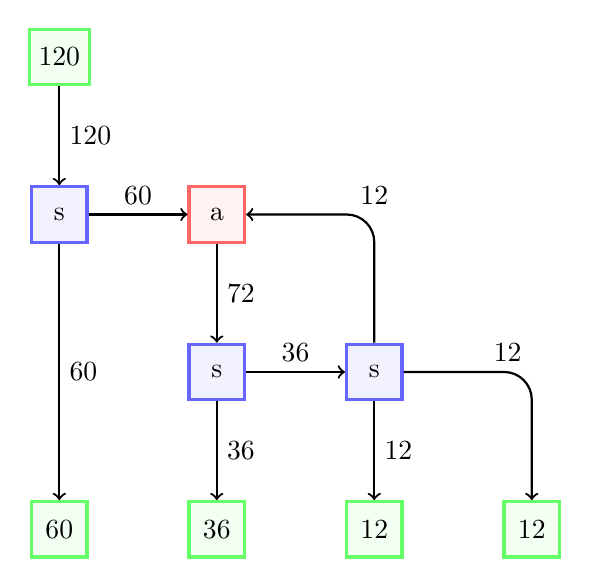
\begin{tikzpicture}[
		s/.style = {rectangle, draw=blue!60,	fill=blue!5,	very thick, minimum size=20},
		a/.style = {rectangle, draw=red!60,		fill=red!5,		very thick, minimum size=20},
		o/.style = {rectangle, draw=green!60,	fill=green!5,	very thick, minimum size=20},
		r/.style = {->, thick, rounded corners=10pt}
		]
		
		
		% === === Nodes === ===
		\node[o]	(in)	at	(0, 4)		{$120$};
		\node[s]	(s)		at	(0, 2)		{s};
		\node[a]	(a)		at	(2, 2)		{a};
		\node[s]	(s1)	at	(2, 0)		{s};
		\node[s]	(s2)	at	(4, 0)		{s};
		\node[o]	(out1)	at	(0, -2)		{$60$};
		\node[o]	(out2)	at	(2, -2)		{$36$};
		\node[o]	(out3)	at	(4, -2)		{$12$};
		\node[o]	(out4)	at	(6, -2)		{$12$};
		
		
		% === === Lines === ===
		\draw[r]	(in.south)	to	node[right]	{$120$}	(s.north);
		\draw[r]	(s.south)	to	node[right]	{$60$}	(out1.north);
		\draw[r]	(s.east)	to	node[above]	{$60$}	(a.west);
		\draw[r]	(a.south)	to	node[right]	{$72$}	(s1.north);
		\draw[r]	(s1.south)	to	node[right]	{$36$}	(out2.north);
		\draw[r]	(s1.east)	to	node[above]	{$36$}	(s2.west);
		\draw[r]	(s2.north)	|-	node[above]	{$12$}	(a.east);
		\draw[r]	(s2.south)	to	node[right]	{$12$}	(out3.north);
		\draw[r]	(s2.east)	-|	node[above left]	{$12$}	(out4.north);
		
		
	\end{tikzpicture}
\end{minipage}
\begin{minipage}{0.5\textwidth}
	\begin{tikzpicture}[
		s/.style = {rectangle, draw=blue!60,	fill=blue!5,	very thick, minimum size=20},
		a/.style = {rectangle, draw=red!60,		fill=red!5,		very thick, minimum size=20},
		o/.style = {rectangle, draw=green!60,	fill=green!5,	very thick, minimum size=20},
		r/.style = {->, thick, rounded corners=10pt},
		r2/.style = {
			line width=1pt, 
			double distance=1pt, 
			arrows = {-Stealth[inset=0pt, angle=45:10pt]},
			rounded corners=10pt,
			red
		},
		]
		
		
		% === === Nodes === ===
		\node[o]	(in)	at	(0, 4)		{$120$};
		\node[s]	(s)		at	(0, 2)		{s};
		\node[a]	(a)		at	(2, 2)		{a};
		\node[s]	(s1)	at	(2, 0)		{s};
		\node[s]	(s2)	at	(4, 0)		{s};
		\node[o]	(out1)	at	(0, -2)		{$70$};
		\node[o]	(out2)	at	(2, -2)		{$30$};
		\node[o]	(out3)	at	(4, -2)		{$10$};
		\node[o]	(out4)	at	(6, -2)		{$10$};
		
		
		% === === Lines === ===
		\draw[r]	(in.south)	to	node[right]	{$120$}	(s.north);
		\draw[r]	(s.south)	to	node[right]	{$70$}	(out1.north);
		\draw[r]	(s.east)	to	node[above]	{$50$}	(a.west);
		\draw[r2]	(a.south)	to	node[right]	{$60$}	(s1.north);
		\draw[r]	(s1.south)	to	node[right]	{$30$}	(out2.north);
		\draw[r]	(s1.east)	to	node[above]	{$30$}	(s2.west);
		\draw[r]	(s2.north)	|-	node[above]	{$10$}	(a.east);
		\draw[r]	(s2.south)	to	node[right]	{$10$}	(out3.north);
		\draw[r]	(s2.east)	-|	node[above left]	{$10$}	(out4.north);
		
		
	\end{tikzpicture}
\end{minipage}





\vspace{0.5in}

Как видим, такая разница происходит из-за того, что ограниченный конвейер подключенн на выход соединителя. Он превращается в тупик по тем же принципам, что и у сплиттера.

\

Однако сдесь у нас 2 \textbf{взаимосвязанных} конвейера заходят в "бутылочное горлышко", так что скорость основного из них стабилизируется, как единственное решение уравнения

\begin{align*}
	&q_0 \cdot \left( 1 - \frac16 \right) = 60 \\
	&q_0 \cdot \frac65 = 60 \\
	&q_0 = 50
\end{align*}


\

Но тут у нас \textbf{единственное} решение -- а если их несколько? рассмотрим пример, в котором у нас несколько \textbf{независимых} входов:




\vspace{0.5in}

\begin{tikzpicture}[
	s/.style = {rectangle, draw=blue!60,	fill=blue!5,	very thick, minimum size=20},
	a/.style = {rectangle, draw=red!60,		fill=red!5,		very thick, minimum size=20},
	o/.style = {rectangle, draw=green!60,	fill=green!5,	very thick, minimum size=20},
	r/.style = {->, thick, rounded corners=10pt},
	r2/.style = {
		line width=1pt, 
		double distance=1pt, 
		arrows = {-Stealth[inset=0pt, angle=45:10pt]},
		rounded corners=10pt,
		red
	},
	]
	
	\draw[fill=black, thick] (-2,5) circle (3pt) node[right] {$\ q>>q_1, q_2$};
	\draw[fill=white, draw=red, thick] (-2,4) circle (3pt) node[right] {$\ q_0 < q_1/2+q_2/2$};
	
	
	% === === Nodes === ===
	\node[o]	(in1)	at	(-2, 2)		{$q_1$};
	\node[o]	(in2)	at	(2, 2)		{$q_2$};
	\node[s]	(s1)	at	(-2, 0)		{s};
	\node[s]	(s2)	at	(2, 0)		{s};
	\node[a]	(a)		at	(0, 0)		{a};
	\node[o]	(out1)	at	(-2, -2)	{$q_1-x$};
	\node[o]	(out2)	at	(0, -2)		{$q_0$};
	\node[o]	(out3)	at	(2, -2)		{$q_2-y$};
	
	
	% === === Lines === ===
	\draw[r]	(in1.south)	to	node[right]	{$q_1$}		(s1.north);
	\draw[r]	(in2.south)	to	node[right]	{$q_2$}		(s2.north);
	\draw[r]	(s1.south)	to	node[right]	{$q_1-x$}	(out1.north);
	\draw[r]	(s2.south)	to	node[right]	{$q_2-x$}	(out3.north);
	\draw[r]	(s1.east)	to	node[above]	{$x$}		(a.west);
	\draw[r]	(s2.west)	to	node[above]	{$y$}		(a.east);
	\draw[r2]	(a.south)	to	node[right]	{$x+y$}		(out2.north);
	
	
\end{tikzpicture}






\vspace{0.5in}

Очень сильно хочется сказать "пускай $x=y$" -- тогда $x = \frac{q_0}2$. Но на деле нам ничто не гарантирует такого: на деле соединитель может приоритезировать один из входов. Второй случай более интересный: например, в satisfactory есть отдельный тип соеденителя -- приоритетный соединитель (англ: priority merger), в котором есть переключатели степени приоритетности того или иного входа.

\

\noindent Пускай левый вход имеет бóльший приоритет. Рассмотрим возможные ситуации:

\begin{itemize}
	\item $\frac{q_1}2 \le q_0$: $x = \frac{q_1}2$, $y = q_0 - \frac{q_1}2$
	
	\item $\frac{q_1}2 \ge q_0$: $x = q_0$, $y = 0$
\end{itemize}






\vspace{0.5in}

\begin{minipage}{0.333\textwidth}
	\begin{tikzpicture}[
		s/.style = {rectangle, draw=blue!60,	fill=blue!5,	very thick, minimum size=15},
		a/.style = {rectangle, draw=red!60,		fill=red!5,		very thick, minimum size=15},
		o/.style = {rectangle, draw=green!60,	fill=green!5,	very thick, minimum size=15},
		r/.style = {->, thick, rounded corners=7.5pt},
		r2/.style = {
			line width=1pt, 
			double distance=1pt, 
			arrows = {-Stealth[inset=0pt, angle=45:10pt]},
			rounded corners=7.5pt,
			red
			},
		]
		
		
		% === === Nodes === ===
		\node[o]	(in1)	at	(-1.5, 1.5)		{$100$};
		\node[o]	(in2)	at	(1.5, 1.5)		{$140$};
		\node[s]	(s1)	at	(-1.5, 0)		{s};
		\node[s]	(s2)	at	(1.5, 0)		{s};
		\node[a]	(a)		at	(0, 0)			{a};
		\node[o]	(out1)	at	(-1.5, -1.5)	{$70$};
		\node[o]	(out2)	at	(0, -1.5)		{$60$};
		\node[o]	(out3)	at	(1.5, -1.5)		{$110$};
		
		
		% === === Lines === ===
		\draw[r]	(in1.south)	to	node[right]	{$100$}		(s1.north);
		\draw[r]	(in2.south)	to	node[right]	{$140$}		(s2.north);
		\draw[r]	(s1.south)	to	node[right]	{$70$}		(out1.north);
		\draw[r]	(s2.south)	to	node[right]	{$110$}		(out3.north);
		\draw[r]	(s1.east)	to	node[above]	{$30$}		(a.west);
		\draw[r]	(s2.west)	to	node[above]	{$30$}		(a.east);
		\draw[r2]	(a.south)	to	node[right]	{$60$}		(out2.north);
		
		
	\end{tikzpicture}
\end{minipage}
\begin{minipage}{0.333\textwidth}
	\begin{tikzpicture}[
		s/.style = {rectangle, draw=blue!60,	fill=blue!5,	very thick, minimum size=15},
		a/.style = {rectangle, draw=red!60,		fill=red!5,		very thick, minimum size=15},
		o/.style = {rectangle, draw=green!60,	fill=green!5,	very thick, minimum size=15},
		r/.style = {->, thick, rounded corners=7.5pt},
		r2/.style = {
			line width=1pt, 
			double distance=1pt, 
			arrows = {-Stealth[inset=0pt, angle=45:10pt]},
			rounded corners=7.5pt,
			red
			},
		]
		
		
		% === === Nodes === ===
		\node[o]	(in1)	at	(-1.5, 1.5)		{$100$};
		\node[o]	(in2)	at	(1.5, 1.5)		{$140$};
		\node[s]	(s1)	at	(-1.5, 0)		{s};
		\node[s]	(s2)	at	(1.5, 0)		{s};
		
		\node[
			draw=red!60, fill=red!5, very thick,
			regular polygon, regular polygon sides=3, 
			rotate=-90, minimum size=0.2cm
			] 
			(tri) at (-0.3, 0) {};
		\node[a]	(a)		at	(0, 0)			{p};
		\node				at	(-0.35, 0)		{$1$};
		
		\node[o]	(out1)	at	(-1.5, -1.5)	{$50$};
		\node[o]	(out2)	at	(0, -1.5)		{$60$};
		\node[o]	(out3)	at	(1.5, -1.5)		{$130$};
		
		
		% === === Lines === ===
		\draw[r]	(in1.south)	to	node[right]	{$100$}		(s1.north);
		\draw[r]	(in2.south)	to	node[right]	{$140$}		(s2.north);
		\draw[r]	(s1.south)	to	node[right]	{$50$}		(out1.north);
		\draw[r]	(s2.south)	to	node[right]	{$130$}		(out3.north);
		\draw[r]	(s1.east)	to	node[above]	{$50$}		(tri.south);
		\draw[r]	(s2.west)	to	node[above]	{$10$}		(a.east);
		\draw[r2]	(a.south)	to	node[right]	{$60$}		(out2.north);
		
		
	\end{tikzpicture}
\end{minipage}
\begin{minipage}{0.333\textwidth}
	\begin{tikzpicture}[
		s/.style = {rectangle, draw=blue!60,	fill=blue!5,	very thick, minimum size=15},
		a/.style = {rectangle, draw=red!60,		fill=red!5,		very thick, minimum size=15},
		o/.style = {rectangle, draw=green!60,	fill=green!5,	very thick, minimum size=15},
		r/.style = {->, thick, rounded corners=7.5pt},
		r2/.style = {
			line width=1pt, 
			double distance=1pt, 
			arrows = {-Stealth[inset=0pt, angle=45:10pt]},
			rounded corners=7.5pt,
			red
			},
		]
		
		
		% === === Nodes === ===
		\node[o]	(in1)	at	(-1.5, 1.5)		{$100$};
		\node[o]	(in2)	at	(1.5, 1.5)		{$140$};
		\node[s]	(s1)	at	(-1.5, 0)		{s};
		\node[s]	(s2)	at	(1.5, 0)		{s};
		
		\node[
			draw=red!60, fill=red!5, very thick,
			regular polygon, regular polygon sides=3, 
			rotate=-90, minimum size=0.2cm
			] 
			(tri) at (-0.3, 0) {};
		\node[a]	(a)		at	(0, 0)			{p};
		\node				at	(-0.35, 0)		{$1$};
		
		\node[o]	(out1)	at	(-1.5, -1.5)	{$70$};
		\node[o]	(out2)	at	(0, -1.5)		{$30$};
		\node[o]	(out3)	at	(1.5, -1.5)		{$140$};
		
		
		
		% === === Lines === ===
		\draw[r]	(in1.south)	to	node[right]	{$100$}		(s1.north);
		\draw[r]	(in2.south)	to	node[right]	{$140$}		(s2.north);
		\draw[r]	(s1.south)	to	node[right]	{$70$}		(out1.north);
		\draw[r]	(s2.south)	to	node[right]	{$140$}		(out3.north);
		\draw[r]	(s1.east)	to	node[above]	{$30$}		(tri.south);
		\draw[r]	(s2.west)	to	node[above]	{$0$}		(a.east);
		\draw[r2]	(a.south)	to	node[right]	{$30$}		(out2.north);
		
		
	\end{tikzpicture}
\end{minipage}












\vspace{0.5in}

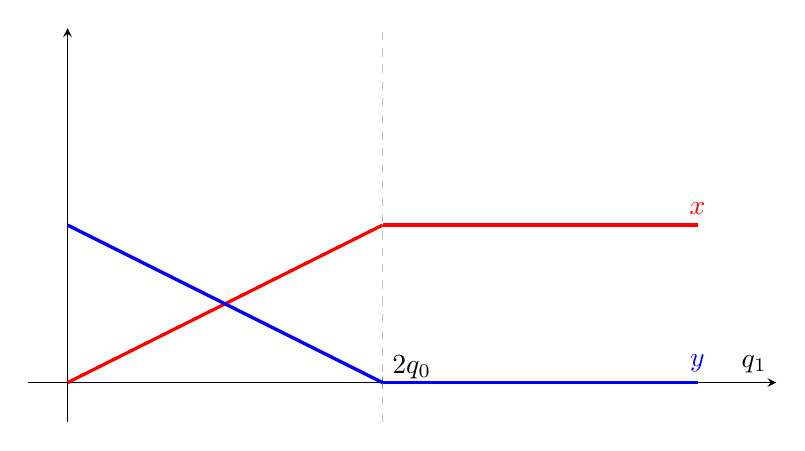
\begin{tikzpicture}
	\begin{axis}[clip = false,
		xmin = -0.5, xmax = 9, ymin = -0.5, ymax = 4.5, xlabel=$q_1$, x=1cm, y=1cm,
		axis lines = middle, xtick = {4},
		xticklabels = {$2q_0$},
		xticklabel style = {anchor=south west}, 
		xmajorgrids = true,
		ytick = {0}, 
		yticklabels = {},
		grid style = dashed]
		
		
		\addplot[domain=0:4, red, very thick]{x/2};
		\addplot[domain=4:8, red, very thick]{2} node[above, pos=1] {$x$};
		
		\addplot[domain=0:4, blue, very thick]{2-x/2};
		\addplot[domain=4:8, blue, very thick]{0} node[above, pos=1] {$y$};
		
	\end{axis}
\end{tikzpicture}









\vspace{0.5in}

Таким образом приоритетный соединитель работает по следующему алгоритму: когда во вход приходит первый ресурс-- он сразу выходит на конвейер $q$. После этого запускается таймер на $1/q$, на протяжении которого никакие ресурсы не выходят, а просто выстраиваютсяв приоритетную очередь. Когда таймер кончается -- ресурс с бóльшим приоритетом выходит, и заново запускается таймер.

\

\noindent По схожему принципу можно реализовать и другие порядки приоретета, если входов больше двух:

\vspace{0.5in}

\begin{minipage}{0.08\textwidth}
	\begin{tikzpicture}[
		a/.style = {rectangle, draw=red!60,		fill=red!5,		very thick, minimum size=20},
		r/.style = {->, thick, rounded corners=10pt},
		]
		
		
		% === === Nodes === ===				
		\node[
			draw=red!60, fill=red!5, very thick,
			regular polygon, regular polygon sides=3, 
			rotate=-90, minimum size=0.8cm
			] 
			(tri) at (-0.4, 0) {};
		\node				at	(-0.5, 0)		{$1$};
		
		\node[
			draw=red!60, fill=red!5, very thick,
			regular polygon, regular polygon sides=3, 
			rotate=180, minimum size=0.8cm
			] 
			(tri) at (0, 0.4) {};
		\node				at	(0, 0.5)		{$2$};
		
		\node[
			draw=red!60, fill=red!5, very thick,
			regular polygon, regular polygon sides=3, 
			rotate=90, minimum size=0.8cm
			] 
			(tri) at (0.4, 0) {};
		\node				at	(0.5, 0)		{$3$};
		
		
		
		\node[a]	(a)		at	(0, 0)			{p};
		
		
		
		
	\end{tikzpicture}
\end{minipage}
\begin{minipage}{0.05\textwidth}
	$$\equiv$$
\end{minipage}
\begin{minipage}{0.333\textwidth}
	\begin{tikzpicture}[
		a/.style = {rectangle, draw=red!60,		fill=red!5,		very thick, minimum size=15},
		o/.style = {rectangle, draw=green!60,	fill=green!5,	very thick, minimum size=15},
		r/.style = {->, thick, rounded corners=7.5pt},
		]
		
		
		% === === Nodes === ===
		\node[
			draw=red!60, fill=red!5, very thick,
			regular polygon, regular polygon sides=3, 
			rotate=-90, minimum size=0.2cm
			] 
					(tri1)	at	(-0.3, 0)		{};
		\node				at	(-0.35, 0)		{$1$};
		\node[a]	(a1)	at	(0, 0)			{p};
		
		
		\node[
			draw=red!60, fill=red!5, very thick,
			regular polygon, regular polygon sides=3, 
			rotate=-90, minimum size=0.2cm
			] 
					(tri2)	at	(-0.3, -1)		{};
		\node				at	(-0.35, -1)		{$1$};
		\node[a]	(a2)	at	(0, -1)			{p};
		
		
		\node[o]	(in1)	at	(-1, 1)			{3};
		\node[o]	(in2)	at	(-1, 0)			{2};
		\node[o]	(in3)	at	(-1, -1)		{1};
		\node[o]	(out)	at	(0, -2)			{out};
		
		
		
		% === === Lines === ===
		\draw[r]	(in1)		-|	(a1.north);
		\draw[r]	(in2)		to	(tri1.south);
		\draw[r]	(a1.south)	to	(a2.north);
		\draw[r]	(in3)		to	(tri2.south);
		\draw[r]	(a2.south)	to	(out.north);
		
	\end{tikzpicture}
\end{minipage}
\begin{minipage}{0.08\textwidth}
	\begin{tikzpicture}[
		a/.style = {rectangle, draw=red!60,		fill=red!5,		very thick, minimum size=20},
		r/.style = {->, thick, rounded corners=10pt},
		]
		
		
		% === === Nodes === ===				
		\node[
			draw=red!60, fill=red!5, very thick,
			regular polygon, regular polygon sides=3, 
			rotate=-90, minimum size=0.8cm
			] 
			(tri) at (-0.4, 1.5) {};
		\node				at	(-0.45, 1.5)	{$1$};
		
		\node[
			draw=red!60, fill=red!5, very thick,
			regular polygon, regular polygon sides=3, 
			rotate=-90, minimum size=0.8cm
			] 
			(tri) at (-0.4, 0.5) {};
		\node				at	(-0.45, 0.5)	{$2$};
		
		\node[
			draw=red!60, fill=red!5, very thick,
			regular polygon, regular polygon sides=3, 
			rotate=-90, minimum size=0.8cm
			] 
			(tri) at (-0.4, -0.5) {};
		\node				at	(-0.45, -0.45)	{$\vdots$};
		
		\node[
			draw=red!60, fill=red!5, very thick,
			regular polygon, regular polygon sides=3, 
			rotate=-90, minimum size=0.8cm
			] 
			(tri) at (-0.4, -1.5) {};
		\node				at	(-0.45, -1.5)	{$n$};
		
		
		
		\draw[draw=red!60, fill=red!5] (-0.333, 2) rectangle node {p} (0.333, -2);
		
		
		
		
	\end{tikzpicture}
\end{minipage}
\begin{minipage}{0.05\textwidth}
	$$\equiv$$
\end{minipage}
\begin{minipage}{0.1\textwidth}
	\begin{tikzpicture}[
		a/.style = {rectangle, draw=red!60,		fill=red!5,		very thick, minimum size=15},
		o/.style = {rectangle, draw=green!60,	fill=green!5,	very thick, minimum size=15},
		r/.style = {->, thick, rounded corners=7.5pt},
		]
		
		
		% === === Nodes === ===
		\node[
			draw=red!60, fill=red!5, very thick,
			regular polygon, regular polygon sides=3, 
			rotate=-90, minimum size=0.2cm
			] 
					(tri1)	at	(-0.3, 0)		{};
		\node				at	(-0.35, 0)		{$1$};
		\node[a]	(a1)	at	(0, 0)			{p};
		
		
		\node[
			draw=red!60, fill=red!5, very thick,
			regular polygon, regular polygon sides=3, 
			rotate=-90, minimum size=0.2cm
			] 
					(tri2)	at	(-0.3, -1)		{};
		\node				at	(-0.35, -1)		{$1$};
		\node[a]	(a2)	at	(0, -1)			{p};
		
		
		\node[
			draw=red!60, fill=red!5, very thick,
			regular polygon, regular polygon sides=3, 
			rotate=-90, minimum size=0.2cm
			] 
					(tri3)	at	(-0.3, -2)		{};
		\node				at	(-0.35, -2)		{$1$};
		\node[a]	(a3)	at	(0, -2)			{p};
		
		
		\node[o]	(in1)	at	(-1, 1)			{$n$};
		\node[o]	(in2)	at	(-1, 0)			{$\vdots$};
		\node[o]	(in3)	at	(-1, -1)		{2};
		\node[o]	(in4)	at	(-1, -2)		{1};
		\node[o]	(out)	at	(0, -3)			{out};
		
		
		
		% === === Lines === ===
		\draw[r]	(in1)	-|	(a1);
		\draw[r]	(in2)	to	(tri1);
		\draw[r]	(a1)	to	(a2);
		\draw[r]	(in3)	to	(tri2);
		\draw[r]	(a2)	to	(a3);
		\draw[r]	(in4)	to	(tri3);
		\draw[r]	(a3)	to	(out);
		
	\end{tikzpicture}
\end{minipage}







\vspace{0.5in}

При этом так же можно добавить приорететный соединитель, который пускает ресурсы только в рамках заданного соотношения $x:y$ по следующему принципу: без ограничений общности положим, что самый первый ресурс зашёл во вход x. Тогда в этом входе запускается таймер на $\frac{x}{x+y} \cdot \frac1{q}$, а на втором, соответственно -- $\frac{y}{x+y} \cdot \frac1{q}$, на время действия которого данный вход превращается в тупик.

\

\noindent Данную схему также можно реализовать при помощи более простых видов соединителей:





\vspace{0.5in}

\begin{minipage}{0.25\textwidth}
	\begin{tikzpicture}[
		s/.style = {rectangle, draw=blue!60,	fill=blue!5,	very thick, minimum size=15},
		a/.style = {rectangle, draw=red!60,		fill=red!5,		very thick, minimum size=15},
		o/.style = {rectangle, draw=green!60,	fill=green!5,	very thick, minimum size=15},
		r/.style = {->, thick, rounded corners=7.5pt},
		r2/.style = {
			line width=1pt, 
			double distance=1pt, 
			arrows = {-Stealth[inset=0pt, angle=45:10pt]},
			rounded corners=7.5pt,
			red
		},
		]
		
		
		% === === Nodes === ===
		\node[o]	(in1)	at	(-1.5, 1.5)		{$120$};
		\node[o]	(in2)	at	(1.5, 1.5)		{$120$};
		\node[s]	(s1)	at	(-1.5, 0)		{s};
		\node[s]	(s2)	at	(1.5, 0)		{s};
		
		\node[
			draw=red!60, fill=red!5, very thick,
			regular polygon, regular polygon sides=3, 
			rotate=-90, minimum size=0.2cm
			] 
					(tri1)	at	(-0.3, 0)		{};
		\node				at	(-0.35, 0)		{$2$};
		
		\node[
			draw=red!60, fill=red!5, very thick,
			regular polygon, regular polygon sides=3, 
			rotate=90, minimum size=0.2cm
			] 
					(tri2)	at	(0.3, 0)		{};
		\node				at	(0.35, 0)		{$1$};
		
		\node[a]	(a)		at	(0, 0)			{:};
		
		\node[o]	(out1)	at	(-1.5, -1.5)	{$80$};
		\node[o]	(out2)	at	(0, -1.5)		{$60$};
		\node[o]	(out3)	at	(1.5, -1.5)		{$100$};
		
		
		
		% === === Lines === ===
		\draw[r]	(in1)	to	node[right]	{$120$}		(s1);
		\draw[r]	(in2)	to	node[right]	{$120$}		(s2);
		\draw[r]	(s1)	to	node[right]	{$80$}		(out1);
		\draw[r]	(s2)	to	node[right]	{$100$}		(out3);
		\draw[r]	(s1)	to	node[above]	{$40$}		(tri1);
		\draw[r]	(s2)	to	node[above]	{$20$}		(tri2);
		\draw[r2]	(a)		to	node[right]	{$60$}		(out2);
		
		
	\end{tikzpicture}
\end{minipage}
\begin{minipage}{0.1\textwidth}
	$$\equiv$$
\end{minipage}
\begin{minipage}{0.333\textwidth}
	\begin{tikzpicture}[
		s/.style = {rectangle, draw=blue!60,	fill=blue!5,	very thick, minimum size=10},
		a/.style = {rectangle, draw=red!60,		fill=red!5,		very thick, minimum size=10},
		o/.style = {rectangle, draw=green!60,	fill=green!5,	very thick, minimum size=10},
		r/.style = {->, thick, rounded corners=5pt},
		r2/.style = {
			line width=1pt, 
			double distance=1pt, 
			arrows = {-Stealth[inset=0pt, angle=45:10pt]},
			rounded corners=7.5pt,
			red
		},
		]
		
		
		% === === Nodes === ===
		\node[o]	(in1)	at	(-2, 1.5)	{$120$};
		\node[o]	(in2)	at	(1, 1.5)	{$120$};
		\node[s]	(s1)	at	(-2, 0)		{s};
		\node[s]	(s2)	at	(1, 0)		{s};
		\node[s] 	(sa)	at	(-1, 0)		{s};
		
		\node[a]	(a)		at	(0, 0)		{a};
		
		\node[o]	(out1)	at	(-2, -1.5)	{$80$};
		\node[o]	(out2)	at	(0, -1.5)	{$60$};
		\node[o]	(out3)	at	(1, -1.5)	{$100$};
		
		
		
		% === === Lines === ===
		\draw[r]	(in1)	to	node[right]	{$120$}		(s1);
		\draw[r]	(in2)	to	node[right]	{$120$}		(s2);
		\draw[r]	(s1)	to	node[right]	{$80$}		(out1);
		\draw[r]	(s2)	to	node[right]	{$100$}		(out3);
		\draw[r]	(s1)	to	node[above]	{$40$}		(sa);
		\draw[r]	(sa)	to	node[above]	{$20$}		(a);
		
		\draw[r]	(sa)	|-	(-0.5, 0.5)	-|	node[above left]	{$20$}	(a);
		
		\draw[r]	(s2)	to	node[above]	{$20$}		(a);
		\draw[r2]	(a)		to	node[right]	{$60$}		(out2);
		
		
	\end{tikzpicture}
\end{minipage}










\vspace{0.667in}

\begin{minipage}{0.34\textwidth}
	\begin{tikzpicture}[
		s/.style = {rectangle, draw=blue!60,	fill=blue!5,	very thick, minimum size=15},
		a/.style = {rectangle, draw=red!60,		fill=red!5,		very thick, minimum size=15},
		o/.style = {rectangle, draw=green!60,	fill=green!5,	very thick, minimum size=15},
		r/.style = {->, thick, rounded corners=7.5pt},
		r2/.style = {
			line width=1pt, 
			double distance=1pt, 
			arrows = {-Stealth[inset=0pt, angle=45:10pt]},
			rounded corners=7.5pt,
			red
		},
		]
		
		
		% === === Nodes === ===
		\node[o]	(in1)	at	(-2, 2)		{$q_1$};
		\node[o]	(in2)	at	(2, 2)		{$q_2$};
		\node[s]	(s1)	at	(-2, 0)		{s};
		\node[s]	(s2)	at	(2, 0)		{s};
		
		\node[
			draw=red!60, fill=red!5, very thick,
			regular polygon, regular polygon sides=3, 
			rotate=-90, minimum size=0.2cm
			] 
					(tri1)	at	(-0.3, 0)	{};
		\node				at	(-0.35, 0)	{$x$};
		
		\node[
			draw=red!60, fill=red!5, very thick,
			regular polygon, regular polygon sides=3, 
			rotate=90, minimum size=0.2cm
			] 
					(tri2)	at	(0.3, 0)	{};
		\node				at	(0.35, 0)	{$y$};
		
		\node[a]	(a)		at	(0, 0)		{:};
		
		\node[o]	(out1)	at	(-2, -2)	{$q_1-\frac{x}{x+y} \cdot q$};
		\node[o]	(out2)	at	(0, -2)		{$q$};
		\node[o]	(out3)	at	(2, -2)		{$q_2-\frac{y}{x+y} \cdot q$};
		
		
		
		% === === Lines === ===
		\draw[r]	(in1)	to	node[left]	{$q_1$}		(s1);
		\draw[r]	(in2)	to	node[right]	{$q_2$}		(s2);
		\draw[r]	(s1)	to	node[left]	{}	(out1);
		\draw[r]	(s2)	to	node[right]	{}	(out3);
		\draw[r]	(s1)	to	node[above]	{$\frac{x}{x+y} \cdot q$}		(tri1);
		\draw[r]	(s2)	to	node[above]	{$\frac{y}{x+y} \cdot q$}		(tri2);
		\draw[r2]	(a)		to	node[right]	{$q$}		(out2);
		
		
	\end{tikzpicture}
\end{minipage}
\begin{minipage}{0.05\textwidth}
	$$\equiv$$
\end{minipage}
\begin{minipage}{0.333\textwidth}
	\begin{tikzpicture}[
		s/.style = {rectangle, draw=blue!60,	fill=blue!5,	very thick, minimum size=10},
		sx/.style ={rectangle, draw=blue!60,	fill=blue!5,	very thick, minimum size=20},
		a/.style = {rectangle, draw=red!60,		fill=red!5,		very thick, minimum size=10},
		o/.style = {rectangle, draw=green!60,	fill=green!5,	very thick, minimum size=10},
		t/.style = {rectangle, draw=black!60,	fill=black!5, 	very thick, minimum size=10},
		r/.style = {->, thick, rounded corners=5pt},
		r2/.style = {
			line width=1pt, 
			double distance=1pt, 
			arrows = {-Stealth[inset=0pt, angle=45:10pt]},
			rounded corners=7.5pt,
			red
		},
		]
		
		
		% === === Nodes === ===
		\node[o]	(in1)	at	(-4, 2)		{$q_1$};
		\node[o]	(in2)	at	(4, 2)		{$q_2$};
		\node[s]	(s1)	at	(-4, 0)		{s};
		\node[s]	(s2)	at	(4, 0)		{s};
		
		\node[sx] 	(s3)	at	(-3, 0)		{S[$x$]};
		\node[t]	(t11)	at	(-2, 2)		{$1$};
		\node[t]	(t12)	at	(-2, 1)		{$2$};
		\node[t]	(t13)	at	(-2, 0)		{$\vdots$};
		\node[t]	(t14)	at	(-2, -1)	{$x$};
		
		\node[sx] 	(s4)	at	(3, 0)		{S[$y$]};
		\node[t]	(t21)	at	(2, 2)		{$1$};
		\node[t]	(t22)	at	(2, 1)		{$2$};
		\node[t]	(t23)	at	(2, 0)		{$\vdots$};
		\node[t]	(t24)	at	(2, -1)		{$y$};
		
		\draw[draw=red!60, fill=red!5] (-0.333, 2.5) rectangle node {a} (0.333, -1.5);
		
		\node[o]	(out1)	at	(-3.5, -3)	{$q_1-\frac{x}{x+y} \cdot q$};
		\node[o]	(out2)	at	(0, -3)		{$q$};
		\node[o]	(out3)	at	(3.5, -3)		{$q_2-\frac{y}{x+y} \cdot q$};
		
		
		
		% === === Lines === ===
		\draw[r]	(in1)	to	node[left]	{$q_1$}				(s1);
		\draw[r]	(in2)	to	node[right]	{$q_2$}				(s2);
		\draw[r]	(s1)	to									(-4, -2.667);
		\draw[r]	(s2)	to									(4, -2.667);
		\draw[r]	(s1)	to									(s3);
		\draw[r]	(s2)	to									(s4);
		
		\draw[r]	(s3)	|-									(t11);
		\draw[r]	(t11)	to	node[above]	{$\frac{q}{x+y}$}	(-0.333, 2);
		\draw[r]	(s3)	|-									(t12);
		\draw[r]	(t12)	to									(-0.333, 1);
		\draw[r]	(s3)	to									(t13);
		\draw[r]	(t13)	to									(-0.333, 0);
		\draw[r]	(s3)	|-									(t14);
		\draw[r]	(t14)	to									(-0.333, -1);
		
		\draw[r]	(s4)	|-									(t21);
		\draw[r]	(t21)	to	node[above]	{$\frac{q}{x+y}$}	(0.333, 2);
		\draw[r]	(s4)	|-									(t22);
		\draw[r]	(t22)	to									(0.333, 1);
		\draw[r]	(s4)	to									(t23);
		\draw[r]	(t23)	to									(0.333, 0);
		\draw[r]	(s4)	|-									(t24);
		\draw[r]	(t24)	to									(0.333, -1);
		
		\draw[r2]	(0, -1.5)	to	node[right]	{$q$}	(out2);
		
		
	\end{tikzpicture}
\end{minipage}














\vspace{0.5in}

\section{Теорема об инверсии}

\

Однако интересно, а что если соединитель не может принять неограниченное количество конвейеров? В реальности как раз так и происходит: в сатисфактори множество числа входов $\mathbb{A} = \{ 2, 3 \}$. 

\

\noindent Теорма: схема для соединителя $(x:y)$ строится, как инверсия отделителя $(x:y)$:

\begin{itemize}
	\item Направление конвейеров реверсируется
	
	\item Соединители заменяются на разъединители
	
	\item Разъединители заменяются на соединители
	
	\item Выходная лента имеет строго ограниченную скорость: $(q < \frac{q_1}2) \land (q < \frac{q_2}2)$
\end{itemize}





\vspace{0.5in}

\begin{minipage}{0.2\textwidth}
	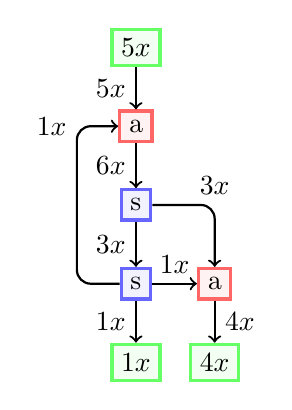
\begin{tikzpicture}[
		s/.style = {rectangle, draw=blue!60, fill=blue!5, very thick, minimum size=10},
		a/.style = {rectangle, draw=red!60, fill=red!5, very thick, minimum size=10},
		o/.style = {rectangle, draw=green!60, fill=green!5, very thick, minimum size=10},
		r/.style = {->, thick, rounded corners=5pt},
		]
		
		%Nodes
		\node[o]	(in)	at	(0, 2)	{$5x$};
		\node[a]	(a1)	at	(0, 1)	{a};
		\node[s]	(s1)	at	(0, 0)	{s};
		\node[s]	(s2)	at	(0, -1)	{s};
		\node[o]	(out1)	at	(0, -2)	{$1x$};
		\node[a]	(a2)	at	(1, -1)	{a};
		\node[o]	(out2)	at	(1, -2)	{$4x$};
		
		%Lines
		\draw[r]	(in) 	to	node[left]	{$5x$}	(a1);
		\draw[r]	(a1)	to	node[left]	{$6x$}	(s1);
		\draw[r]	(s1)	to	node[left]	{$3x$}	(s2);
		\draw[r]	(s1)	-|	node[above]	{$3x$}	(a2);
		\draw[r]	(s2)	to	node[above]	{$1x$}	(a2);
		\draw[r]	(s2)	-| (-0.75, 0) |- node[left]	{$1x$}	(a1);
		\draw[r]	(s2)	to	node[left]	{$1x$}	(out1);
		\draw[r]	(a2)	to	node[right]	{$4x$}	(out2);
		
	\end{tikzpicture}
\end{minipage}
\begin{minipage}{0.15\textwidth}
	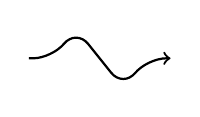
\begin{tikzpicture}[
		r/.style = {->, thick, rounded corners=7pt},
		]
		
		\draw[r] (-0.6, 0) to (-0.3, 0) to (0, 0.375) to (0.6, -0.375) to (0.9, 0) to (1.2, 0);
		
	\end{tikzpicture}
\end{minipage}
\begin{minipage}{0.2\textwidth}
	\begin{tikzpicture}[
		s/.style = {rectangle, draw=blue!60, fill=blue!5, very thick, minimum size=10},
		a/.style = {rectangle, draw=red!60, fill=red!5, very thick, minimum size=10},
		o/.style = {rectangle, draw=green!60, fill=green!5, very thick, minimum size=10},
		r/.style = {->, thick, rounded corners=5pt},
		r1/.style = {<-, thick, rounded corners=5pt},
		r2/.style = {
			line width=0.6pt, 
			double distance=0.6pt, 
			arrows = {-Stealth[inset=0pt, angle=45:6pt]},
			rounded corners=5pt,
			red
		},
		]
		
		\node[right] (1) at (4, 2) {$1x < \frac{q_1}2 \ , \ 4x < \frac{q_2}2$};
		\draw[fill=black, thick] (4,1) circle (3pt) node[right] {$\ q>>q_1, q_2$};
		\draw[fill=white, draw=red, thick] (4,0) circle (3pt) node[right] {$\ q_0 < q_1/2, q_2/2$};
		
		
		%Nodes
		\node[o]	(in)	at	(0, 2)	{$5x$};
		\node[s]	(a1)	at	(0, 1)	{s};
		\node[a]	(s1)	at	(0, 0)	{a};
		\node[a]	(s2)	at	(0, -1)	{a};
		\node[s]	(out1)	at	(0, -2)	{s};
		\node[s]	(a2)	at	(1, -1)	{s};
		\node[s]	(out2)	at	(1, -2)	{s};
		\node[o]	(in1)	at	(0, -3)	{$q_1$};
		\node[o]	(in2)	at	(1, -3)	{$q_2$};
		\node[o]	(out3)	at	(-2, 2)	{$q_1-x$};
		\node[o]	(out4)	at	(2, 2)	{$q_2-4x$};
		
		
		%Lines
		\draw[r2]	(a1) 	to	node[left]	{$5x$}	(in);
		\draw[r1]	(a1)	to	node[left]	{$6x$}	(s1);
		\draw[r1]	(s1)	to	node[left]	{$3x$}	(s2);
		\draw[r1]	(s1)	-|	node[above]	{$3x$}	(a2);
		\draw[r1]	(s2)	to	node[above]	{$1x$}	(a2);
		\draw[r1]	(s2)	-| (-0.75, 0) |- node[left]	{$1x$}	(a1);
		\draw[r1]	(s2)	to	node[left]	{$1x$}	(out1);
		\draw[r1]	(a2)	to	node[right]	{$4x$}	(out2);
		\draw[r]	(in1)	to	node[left]	{$1x$}	(out1);
		\draw[r]	(in2)	to	node[right]	{$4x$}	(out2);
		\draw[r]	(out1)	-|						(out3);
		\draw[r]	(out2)	-|						(out4);
		
	\end{tikzpicture}
\end{minipage}









\vspace{0.5in}

Как можем заметить, в такой схеме сохраняются даже пропускные способности. При этом разъединители перестают в обязательном порядке делить поровну, поскольку они становятся образом соединителей, которые могут принимать конвейеры в любых соотношениях.

\

Нетрудно понять, что если $\mathbb{A} \not\supset \mathbb{T}$ -- то такое преобразование в прямом виде -- невозможно. Но на основе этого принципа можно построить искомую схему. Обозначим: $s(x+y) = s$, $s - (x+y) = b$, $k\cdot(x+y)$. Реализуем схему для соединения $x+y$ конвейеров, а затем реализуем подсхемы для разделения на $x$, $y$ и $b$ независимо. Так же понадобится промежуточно реализоавть схему для разделения на $2$ (если $2 \not\in \mathbb{T}$):






\newpage

\begin{tikzpicture}[
	s`/.style =	{rectangle,	draw=blue!60,	fill=blue!5,	very thick, minimum size=20},
	s/.style =	{rectangle,	draw=blue!60,	fill=blue!5,	very thick, minimum size=10},
	a/.style =	{rectangle,	draw=red!60,	fill=red!5,		very thick, minimum size=10},
	o/.style =	{rectangle,	draw=green!60,	fill=green!5,	very thick, minimum size=10},
	t/.style =	{rectangle,	draw=black!60,	fill=black!5,	thick, 		minimum size=10, inner sep=1pt},
	r`/.style =	{<-, thick, rounded corners=5pt},
	r/.style =	{->, thick, rounded corners=5pt},
	r2/.style = {
		line width=1pt, 
		double distance=1pt, 
		arrows = {-Stealth[inset=0pt, angle=45:10pt]},
		rounded corners=7.5pt,
		red
	},
	]
	
	% === === Nodes === ===
	\node[o]	(in)	at	(-6, 0)		{$v$};
	\node[s`]	(a1)	at	(-3, 0)		{S[$2$]};
	
	\node[a]	(s1)	at	(-1.75, 0)	{a};
	\node[t]	(t11)	at	(-0.75, 0)	{$1$};
	\node[t]	(t12)	at	(-0.75, -4)	{$2$};
	\node[t]	(t1i)	at	(-0.75, -9)	{$a_{i_1}$};
	
	\node[a]	(s11)	at	(0, 0)		{a};
	\node[t]	(t121)	at	(1, 0)		{$1$};
	\node[t]	(t122)	at	(1, -1)		{$2$};
	\node[t]	(t12e)	at	(1, -2)		{$\vdots$};
	\node[t]	(t12i)	at	(1, -3)		{$a_{i_2}$};
	
	\node[a]	(s21)	at	(0, -4)		{a};
	\node[t]	(t221)	at	(1, -4)		{$1$};
	\node[t]	(t222)	at	(1, -5)		{$2$};
	\node[t]	(t22e)	at	(1, -6)		{$\vdots$};
	\node[t]	(t22i)	at	(1, -7)		{$a_{i_2}$};
	
	\node[a]	(si1)	at	(0, -9)		{a};
	\node[t]	(ti21)	at	(1, -9)		{$1$};
	\node[t]	(ti22)	at	(1, -10)	{$2$};
	\node[t]	(ti2e)	at	(1, -11)	{$\vdots$};
	\node[t]	(ti2i)	at	(1, -12)	{$a_{i_2}$};		
	
	% === === etc === ===
	\draw[draw=red!60,		fill=red!5]		(1.5, 0.5)	rectangle node {$\ldots$} (2, -12.5);
	\draw[draw=black!60,	fill=black!5]	(-1, -7.75)	rectangle node {$\ldots$} (1.25, -8.25);
	
	\node[t]	(t1)	at	(2.5, 0)		{$1$};
	\node[t]	(t2)	at	(2.5, -2)		{$2$};
	\node[t]	(te1)	at	(2.5, -4)		{$\vdots$};
	\node[t]	(tb)	at	(2.5, -6)		{$b$};
	\node[t]	(tb+)	at	(2.7, -8)		{$b+1$};
	\node[t]	(te2)	at	(2.5, -10.2)	{$\vdots$};
	\node[t]	(tn)	at	(2.5, -12)		{$s$};
	
	\node[s`]	(a2)	at	(3, -3)			{S[$b$]};
	\node[t]	(t1`x)	at	(5.5, 0)		{$1$};
	\node[t]	(t2`x)	at	(5.5, -1.7)		{$2$};
	\node[t]	(te`x)	at	(5.5, -3.4)		{$\ldots$};
	\node[t]	(tx)	at	(5.5, -5.1)		{$x$};
	\node[t]	(t1`y)	at	(5.5, -6.8)		{$1$};
	\node[t]	(t2`y)	at	(5.5, -8.5)		{$2$};
	\node[t]	(te`y)	at	(5.5, -10.2)	{$\ldots$};
	\node[t]	(ty)	at	(5.5, -12)		{$y$};
	
	\node[s`]	(ax)	at	(6.5, -2.55)	{S[$x$]};
	\node[s`]	(ay)	at	(6.5, -9.35)	{S[$y$]};
	
	\node[s]	(sx)	at	(8, -2.55)		{s};
	\node[s]	(sy)	at	(8, -9.35)		{s};
	
	\node[o]	(outx)	at	(-6, 2)			{$kx+q_1$};
	\node[o]	(outy)	at	(-6, -2)		{$ky+q_2$};
	
	\node[o]	(inx)	at	(9.5, -2.55)	{$2kx+q_1$};
	\node[o]	(iny)	at	(9.5, -9.35)	{$2ky+q_2$};
	
	
	
	% === === Lines === ===
	\draw[r2]	(a1)		to	node[above]	{$v$}	(in);
	\draw[r`]	(a1)		to	(s1);
	
	\draw[r`]	(s1)		to	(t11);
	\draw[r`]	(s1)		|-	(t12);
	\draw[r`]	(s1)		|-	(-1, -8);
	\draw[r`]	(s1)		|-	(t1i);
	
	\draw[r`]	(t11)		to	(s11);
	\draw[r`]	(s11)		to	(t121);
	\draw[r`]	(s11)		|-	(t122);
	\draw[r`]	(s11)		|-	(t12e);
	\draw[r`]	(s11)		|-	(t12i);
	
	\draw[r`]	(t12)		to	(s21);
	\draw[r`]	(s21)		to	(t221);
	\draw[r`]	(s21)		|-	(t222);
	\draw[r`]	(s21)		|-	(t22e);
	\draw[r`]	(s21)		|-	(t22i);
	
	\draw[r`]	(t1i)		to	(si1);
	\draw[r`]	(si1)		to	(ti21);
	\draw[r`]	(si1)		|-	(ti22);
	\draw[r`]	(si1)		|-	(ti2e);
	\draw[r`]	(si1)		|-	(ti2i);
	
	\draw[r`]	(t121)		to	(1.5, 0);
	\draw[r`]	(t122)		to	(1.5, -1);
	\draw[r`]	(t12e)		to	(1.5, -2);
	\draw[r`]	(t12i)		to	(1.5, -3);
	\draw[r`]	(t221)		to	(1.5, -4);
	\draw[r`]	(t222)		to	(1.5, -5);
	\draw[r`]	(t22e)		to	(1.5, -6);
	\draw[r`]	(t22i)		to	(1.5, -7);
	\draw[r`]	(1.25, -8)	to	(1.5, -8);
	\draw[r`]	(ti21)		to	(1.5, -9);
	\draw[r`]	(ti22)		to	(1.5, -10);
	\draw[r`]	(ti2e)		to	(1.5, -11);
	\draw[r`]	(ti2i)		to	(1.5, -12);
	
	\draw[r`]	(2, 0)		to	(t1);
	\draw[r`]	(2, -2)		to	(t2);
	\draw[r`]	(2, -4)		to	(te1);
	\draw[r`]	(2, -6)		to	(tb);
	\draw[r`]	(2, -8)		to	(tb+);
	\draw[r`]	(2, -10.2)	to	(te2);
	\draw[r`]	(2, -12)	to	(tn);
	
	\draw[r`]	(t1) 		-| 	(a2);
	\draw[r`]	(t2) 		-| 	(a2);
	\draw[r`]	(te1)		-| 	(a2);
	\draw[r`]	(tb)		-| 	(a2);
	
	\draw[r`] 	(a2)		-| 	(4, 1) 		-| (a1);
	
	\draw[r`]	(tb+)		to 	(4.5, -8) 	|- 	(t1`x);
	\draw[r`]	(te2)		to 	(5, -10.2)	|- 	(t2`x);
	\draw[r`]	(te2)		to	(5, -10.2)	|- 	(te`x);
	\draw[r`]	(te2)		to	(5, -10.2)	|-	(tx);
	\draw[r`]	(te2)		to 	(5, -10.2) 	|- 	(t1`y);
	\draw[r`]	(te2)		to 	(5, -10.2)	|- 	(t2`y);
	\draw[r`]	(te2)		to	(te`y);
	\draw[r`]	(tn)		to	(ty);
	
	\draw[r`]	(t1`x)		-|	(ax);
	\draw[r`]	(t2`x)		-|	(ax);
	\draw[r`]	(te`x)		-|	(ax);
	\draw[r`]	(tx)		-|	(ax);
	\draw[r`]	(t1`y)		-|	(ay);
	\draw[r`]	(t2`y)		-|	(ay);
	\draw[r`]	(te`y)		-|	(ay);
	\draw[r`]	(ty)		-|	(ay);
	
	\draw[r`]	(ax)		to	node[above]	{$kx$}	(sx);
	\draw[r`]	(ay)		to	node[above]	{$ky$}	(sy);
	
	\draw[r]	(inx)		to	(sx);
	\draw[r]	(iny)		to	(sy);
	
	\draw[r]	(sx)		|-	(outx);
	\draw[r]	(sy)		|-	(6.5, -13)	-|	(-3, -2)	to	(outy);
	
\end{tikzpicture}








\vspace{0.5in}

Казалось бы, что данная схема очень громоздкая, ведь содержит аш 5 различных подсхем... Наделе все 5, включая схему соединителя -- можно сократить по ранее упомянтм же принципам "ёлочки" и "палочки". А если для какого-нибудь $\alpha \in \{ x, y, b \} \ : \ \exists \ t \in \mathbb{T} \ | \ \alpha < t$ -- то такую схему можно реализовать даже без вовзрата, а с уже известными нам тупиками.

\

Хорошо, схема может и не такая уж и большая, как кажется -- но какой всё же в ней смысл, если для каждых $q_1$ и $q_2$ можно реализовать свой разделитель? Вот именно, что \underline{для каждых $q_1$ и $q_2$} нужно будет реализовывать отдельную схему, а тут -- одна для всех. Например, если ресурсы перевозятся поездами с некоторой задержкой с разных производств на другие разные производства -- то одну эту схему можно использовать для разделения обоих случаев, а не строить две независимые схемы -- Нужно лишь в конце тем, или иным методом сделать распределитель на разные заводы (чем мы займёмся в дальнейших главах).










\vspace{0.5in}

\section{Затворы}

\

Однако важно учесть, что может быть так, что $k\cdot(x+y) \not\in \mathbb{V}$. Обозначив $k\cdot(x+y) = v$. Рассмотрим три возможные ситуации:

\

Если $v < \min(\mathbb{V})$ -- запора происходить не будет, и ресурсы будут просто проскальзывать, и соотношение перестанет сохранятся. Можно реализовать затворный механизм: реализуем схему на возврат некоторой доли $\frac{a}{b}$, а оставшиеся конвейеры соеденим. Тогда необходимо, чтобы:

\

$$
v \cdot \frac{1}{1-\frac{a}{b}} = \min(\mathbb{V})
\quad \quad
\frac{v}{\min(\mathbb{V})} = 1 - \frac{a}{b}
\quad \quad
\frac{a}{b} = \frac{\min(\mathbb{V}) - v}{\min(\mathbb{V})}
$$

$$
a = \frac{\min(\mathbb{V}) - v}{\gcd(\min(\mathbb{V}), v)}
\ , \
b = \frac{\min(\mathbb{V})}{\gcd(\min(\mathbb{V}), v)}
$$



\vspace{0.5in}

\begin{tikzpicture}[
	s/.style = {rectangle, draw=blue!60,	fill=blue!5,	very thick, minimum size=20},
	a/.style = {rectangle, draw=red!60,		fill=red!5,		very thick, minimum size=20},
	o/.style = {rectangle, draw=green!60,	fill=green!5,	very thick, minimum size=20},
	r/.style = {->, thick, rounded corners=10pt},
	r2/.style = {
		line width=1pt, 
		double distance=1pt, 
		arrows = {-Stealth[inset=0pt, angle=45:10pt]},
		rounded corners=10pt,
		red
	},
	]
	
	
	% === === Nodes === ===
	\node[o]	(in)	at	(-4, 0)		{$10$};
	\node[a]	(a1)	at	(-2, 0)		{a};
	\node[s]	(s1)	at	(0, 0)		{s};
	\node[s]	(s2)	at	(2, 0)		{s};
	\node[a]	(a2)	at	(2, 2)		{a};
	\node[o]	(out)	at	(4, -2)		{$10$};
	
	
	
	% === === Lines === ===
	\draw[r]	(in)	to	node[above]			{$10$}	(a1);
	\draw[r2]	(a1)	to	node[above]			{$60$}	(s1);
	\draw[r]	(s1)	to	node[above]			{$30$}	(s2);
	\draw[r]	(s1)	|-	node[above right]	{$30$}	(a2);
	\draw[r]	(s2)	to	node[left]			{$10$}	(a2);
	
	\draw[r]	(s2)	-|	(3, 1)	|-	node[below right]	{$10$}	(a2);
	\draw[r]	(a2)	|-	(0, 3)	-|	node[above right]	{$50$}	(a1);
	
	\draw[r]	(s2)	|-	node[below right]	{$10$}	(out);
	
\end{tikzpicture}








\vspace{0.5in}

Если же $v > \max(\mathbb{V})$ -- то наоборот будет происходить перезапор: соотношение будет сохраняться, но числа на выходах будут другие. Воспользуемя принципом чайника и аксиомой архимеда, и просто разделим входной конвейер на несколько параллельных частей, в каждой из которых $\exists \ u \in \mathbb{V} \ | \ v < u$, к которому применим затворный механизм:

\vspace{0.5in}

\begin{tikzpicture}[
	s/.style = {rectangle, draw=blue!60,	fill=blue!5,	very thick, minimum size=10},
	a/.style = {rectangle, draw=red!60,		fill=red!5,		very thick, minimum size=10},
	o/.style = {rectangle, draw=green!60,	fill=green!5,	very thick, minimum size=10},
	r/.style = {->, thick, rounded corners=5pt},
	r2/.style = {
		line width=1pt, 
		double distance=1pt, 
		arrows = {-Stealth[inset=0pt, angle=45:10pt]},
		rounded corners=7.5pt,
		red
	},
	]
	
	
	% === === Nodes === ===
	\node[s]	(s)		at	(-2, -2)	{s};
	\node[o]	(in)	at	(-4, -2)	{$100$};
	
	\node[a]	(a11)	at	(-1, 0)		{a};
	\node[s]	(s11)	at	(0, 0)		{s};
	\node[s]	(s21)	at	(1, 0)		{s};
	\node[a]	(a21)	at	(1, -1)		{a};
	
	\node[a]	(a12)	at	(-1, -4)	{a};
	\node[s]	(s12)	at	(0, -4)		{s};
	\node[s]	(s22)	at	(1, -4)		{s};
	\node[a]	(a22)	at	(1, -3)		{a};
	
	\node[a]	(a3)	at	(1, -2)		{a};
	\node[o]	(out)	at	(3, -2)		{$100$};
		
	
	
	% === === Lines === ===
	\draw[r]	(in)	to	node[above]			{$100$}	(s);
	\draw[r]	(s)		|-	node[below left]	{$50$}	(a11);
	\draw[r]	(s)		|-	node[above left]	{$50$}	(a12);
	
	
	\draw[r2]	(a11)	to	node[above]			{$60$}	(s11);
	\draw[r]	(s11)	to	node[above]			{$30$}	(s21);
	\draw[r]	(s11)	|-	node[above right]	{$30$}	(a21);
	\draw[r]	(s21)	to	node[left]			{$10$}	(a21);
	
	\draw[r]	(s21)	-|	(1.5, -0.5)	|-	node[above right]	{$10$}	(a21);
	\draw[r]	(s21)	|-	(0, 0.5)	-|	node[above right]	{$10$}	(a11);
	
	\draw[r]	(a21)	to	node[left]			{$50$}	(a3);
	
	
	\draw[r2]	(a12)	to	node[above]			{$60$}	(s12);
	\draw[r]	(s12)	to	node[above]			{$30$}	(s22);
	\draw[r]	(s12)	|-	node[above right]	{$30$}	(a22);
	\draw[r]	(s22)	to	node[left]			{$10$}	(a22);
	
	\draw[r]	(s22)	-|	(1.5, -3.5)	|-	node[below right]	{$10$}	(a22);
	\draw[r]	(s22)	|-	(0, -4.5)	-|	node[below right]	{$10$}	(a12);
	
	
	\draw[r]	(a22)	to	node[left]			{$50$}	(a3);
	\draw[r]	(a3)	to	node[above]			{$100$}	(out);
	
\end{tikzpicture}








\vspace{0.5in}

Последняя ситуация: если $\exists \ m, M \in \mathbb{V} \ | \ m < v < M$ -- то в зависимости от конвретных значений $v$ и $\mathbb{V}$ можно использовать оба предыдущих метода.








































































































